 \documentclass[t,14pt]{beamer}
 %
 % Packages pour le français
 \usepackage[T1]{fontenc} 
 \usepackage[utf8]{inputenc}
 \usepackage[frenchb]{babel}
 %
 % pour un pdf lisible à l'écran
 % il y a d'autres choix possibles 
 \usepackage{pslatex}
\usetheme{Singapore}
  \usecolortheme{rose}
  \setbeamertemplate{blocks}[rounded][shadow=true]

\title{\textbf{\textit{Extraction et Analyse d'Images}}}
\subtitle{PED}
\author{\scriptsize{Manson Tomy\\
		Mestreau Nicolas\\
		Ridel Fabien\\
		Wen Jun\\
		\vspace{10mm}
		Encadrant : \\
		Laviole Jérémy\\
		}}
\institute{\tiny Université de Bordeaux 1}



\begin{document}

\frame{\titlepage}

%% part 1 - Jun
\section[Présentation]{Présentation}
\AtBeginSection[]{
\begin{frame}{Table des matières}
\small \tableofcontents[currentsection, hideothersubsections]
\end{frame}
}

\begin{frame}{Présentation du projet}
\begin{center}
\vspace{5mm}
Le but de ce projet est la création d'une bibliothèque d'analyse d'image.

\end{center}
\begin{itemize}
\item Entrée : un flux vidéo de dessin ou des images de haute qualité.
\item Analyse : détection de pictogrammes ou extraction de nouveauté.
\item Sortie : une image de pictogrammes avec les détections ou les nouveautés d'une image.
\end{itemize}
\end{frame}

\begin{frame}{Objectifs}
\vspace{5mm}
\begin{block}{}
\begin{itemize}
\item Améliorer la qualité de l'image.
\item Détecter les formes simples. 
\item Récupérer les nouveautés du dessin.
\end{itemize}
\end{block}
\begin{center}
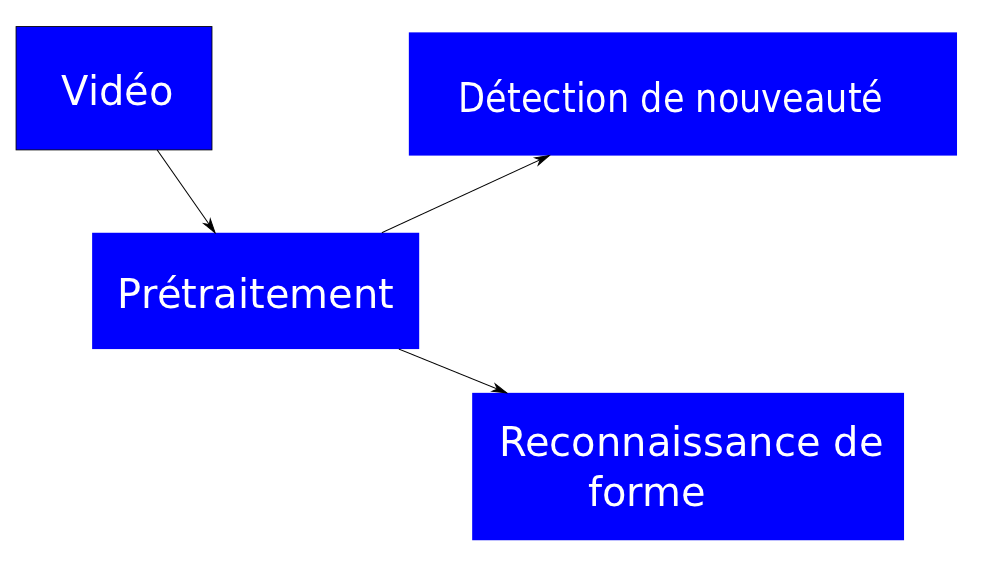
\includegraphics[scale=0.2]{images/dessin.png} 
\\ schéma de processus
\end{center}
\end{frame}


\begin{frame}{Applications Possibles}
\vspace{2mm}
\begin{itemize}
\item Jeu vidéo en Réalité Augmentée

\begin{center}
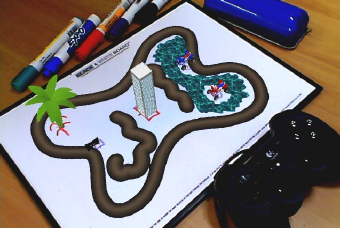
\includegraphics[scale=0.5]{images/sketchchasser.png}
\textit{\\sketchchasser}
\end{center}
\item Auto-scanner 
\end{itemize}
\end{frame}

%% part 2 - Fabien
\section[Pré-traitement]{Pré-traitement}
\begin{frame}{Objectif}
\vspace{5mm}
\begin{block}{}
Améliorer la qualité de l'image.
\end{block}
\begin{itemize}[<+->]
\item Réduire le bruit de l'image.
\item Segmenter l'image : binarisation.

%La segmentation se résume à une binarisation, 

%Binarisation deux classes; une pour le fond et une pour l'objet.  

\item Problème difficile pour un dessin avec une vidéo de basse qualité 
%:  segmentation de dessin avec une vidéo de basse qualité est un problème difficile.





\end{itemize}
\end{frame}

\vspace{5mm}
\begin{frame}{Difficultés}
\vspace{5mm}
\begin{block}{}
Éclairage non uniforme.
\end{block}
\begin{center}
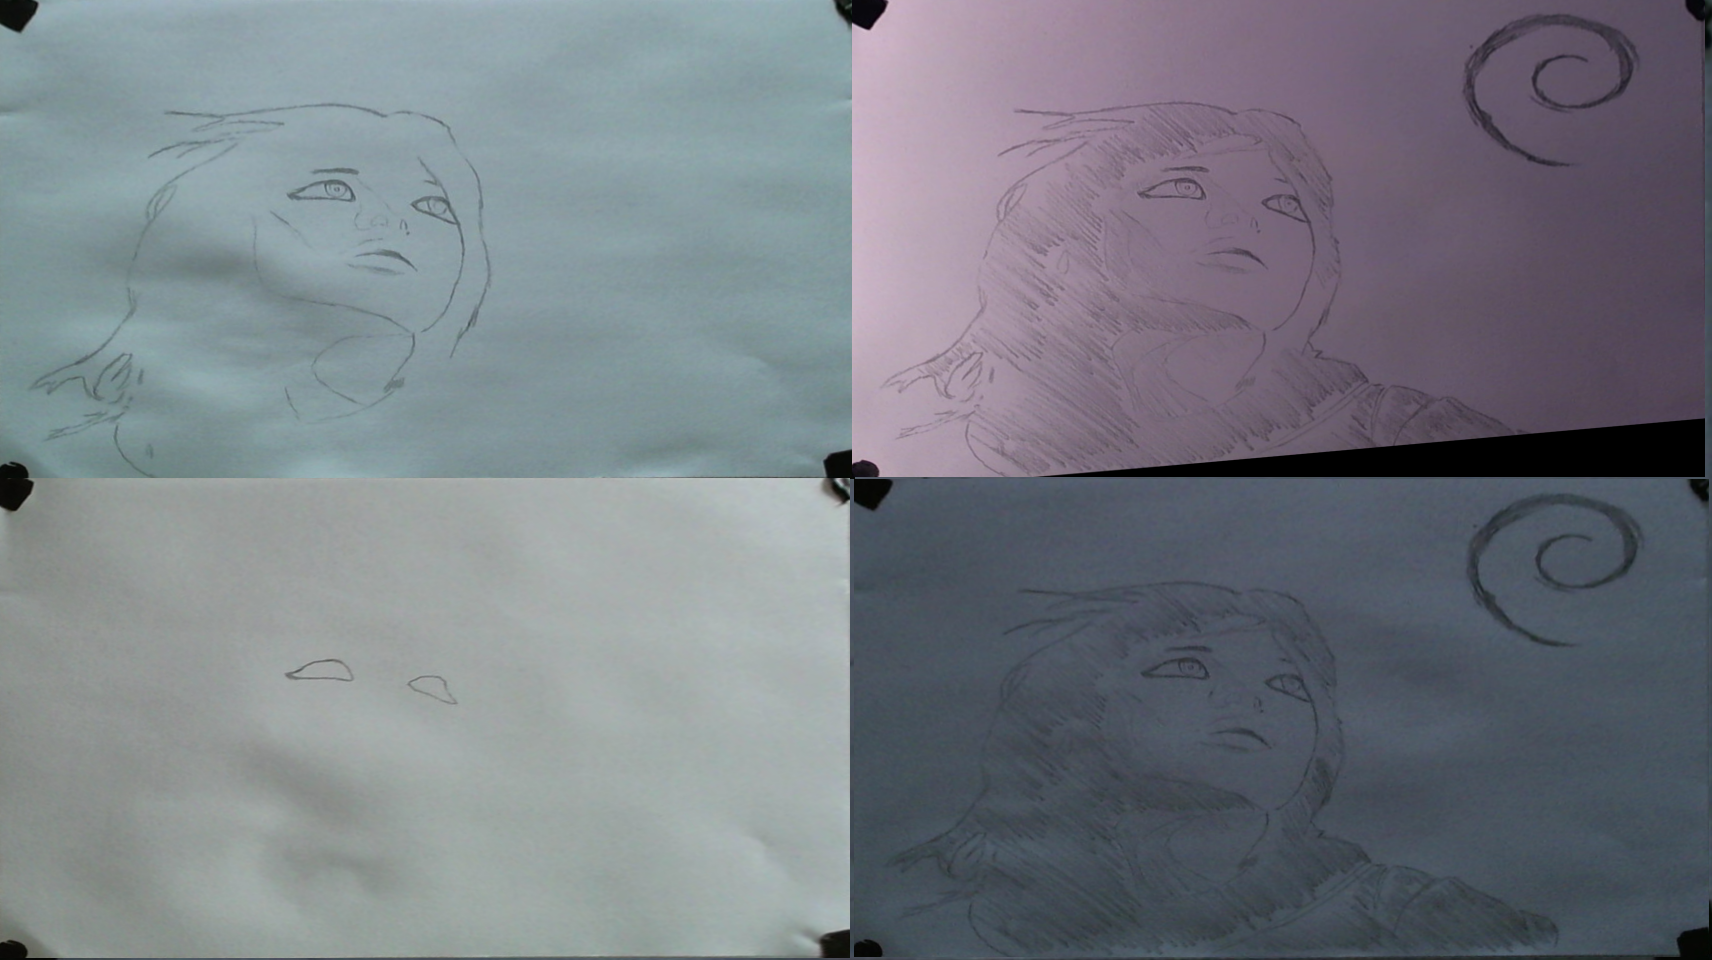
\includegraphics[scale=0.20]{images/diffEclairage.png}
\end{center}
\end{frame}
%Seuillage globale qui naïvement semble être la bonne solution, montre ses limites la %vidéo peut entraîné un éclairage non uniforme.

\begin{frame}{Difficultés}
\vspace{5mm}
\begin{block}{}
Zones homogènes (coloriées).
\end{block}
\begin{center}
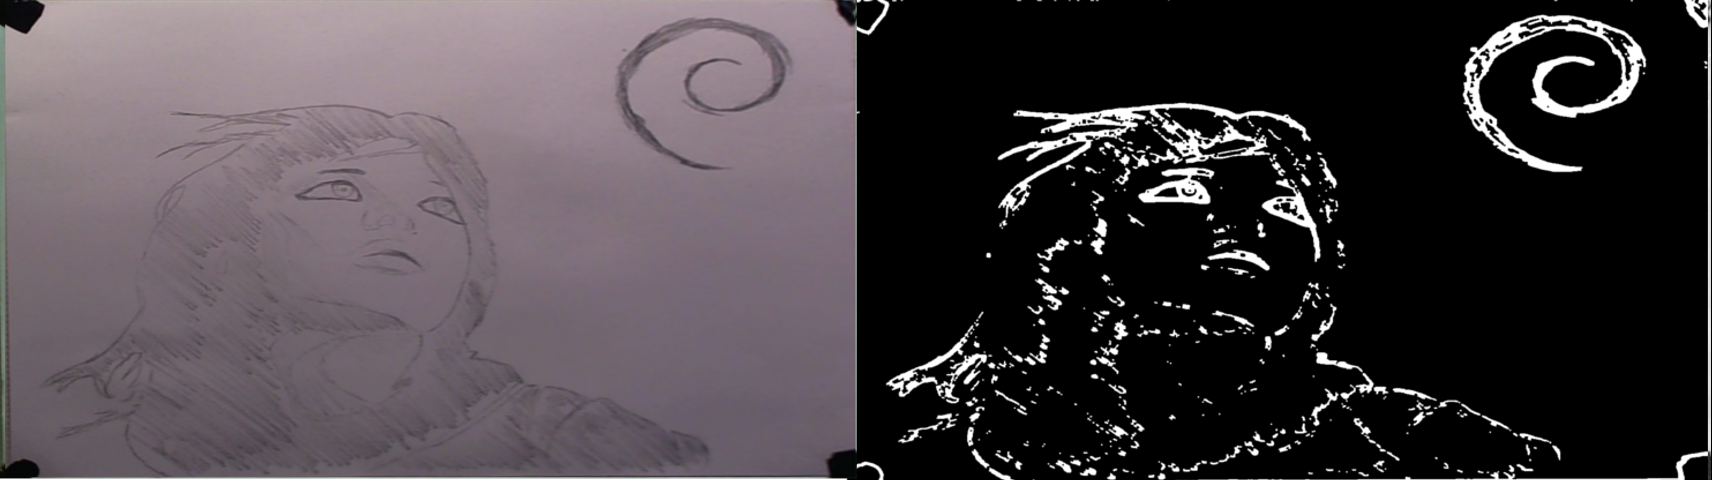
\includegraphics[width=\textwidth]{images/sobel.png}
\end{center}

%Un dessin est définit par un ensemble de trait et dans certain cas des zones %homogènes( coloriées) ce qui ne nous permet pas d'utiliser un filtre de détection de %contour. ce qui peut etre optimale pour un simple ensemble de trait  
\end{frame}

\begin{frame}{Méthodes utilisées}
\vspace{5mm}
\begin{block}{}
Balance des blancs.
\end{block}
\begin{center}
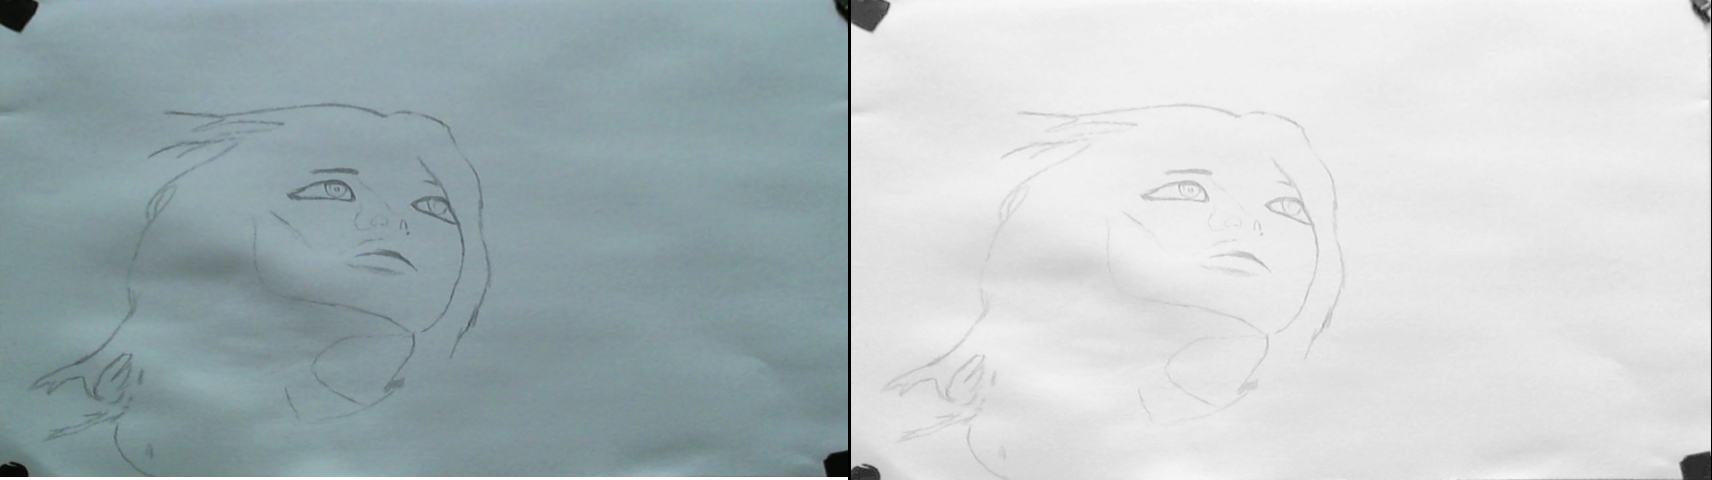
\includegraphics[width=\textwidth]{images/wb.png}
\end{center}
\end{frame}
%étirement d'histogramme sur chaques canals avant de les rassembler ==> 
%permet d'augmenter le contraste.
\begin{frame}{Méthodes utilisées}
\vspace{5mm}
\begin{block}{}
Seuillage local (Méthode de Sauvola) 
\end{block}
\begin{center}
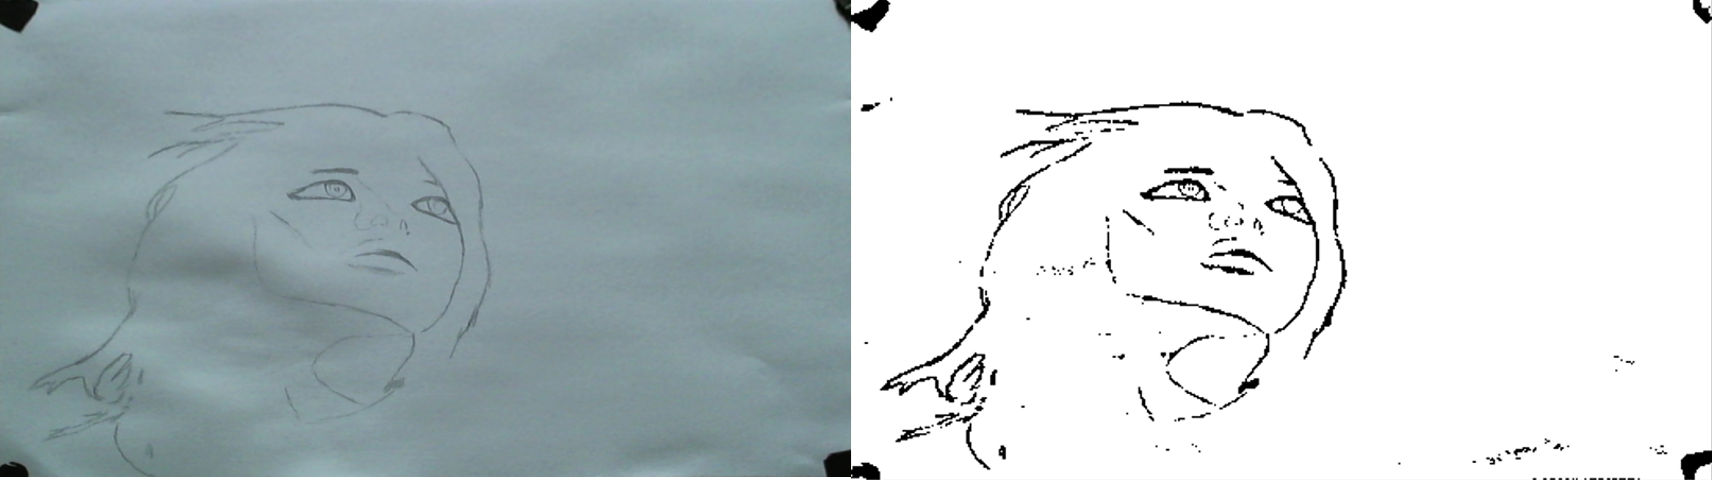
\includegraphics[width=\textwidth]{images/sauvola.png}
\end{center}
%étude de l'article ... compare les méthodes de binarisation  
%formule 
%difficulté trait de faible intensité,  
\end{frame}

%\vspace{5mm}
%\begin{frame}{Sauvola}
%\vspace{5mm}
%
%\begin{equation}
%	S(i,j) = \mu(i,j) + \kappa.((\sigma(i,j)/R)-1))
%\end{equation}
%
%Avec :
%- S(i, j) : seuil à appliquer pour le point i, j ;\\
%- $\sigma(i, j)$ : valeur de l’écart type dans une fenêtre centré en i, j de taille $N * M$ ;\\
%- $\mu(i, j)$ : valeur moyenne des niveaux de gris dans la même fenêtre ;\\
%- $\kappa$ : constante fixée le plus généralement à 0, 2 ;\\
%- R : constante permettant d'ajuster la dynamique de l'ecart type, géneralement 128.
%- N et M appartenant à N.\\
%%article de ...
%%permet d'obtenir la moyenne en 2 additions et deux soustractions
%
%\end{frame}

\begin{frame}{Optimisation}
\vspace{5mm}
\begin{block}{}
Image intégrale
\end{block}
Reformulation par Viola et Jones "Robust real-time face detection" 2004\\
\begin{center}
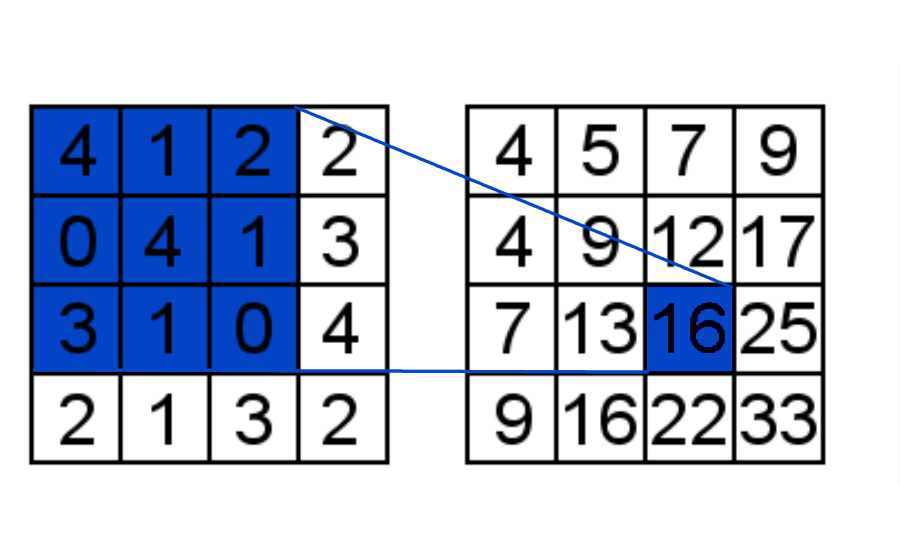
\includegraphics[width=0.5\textwidth]{images/imageIntegrale1.png}
\end{center}
\end{frame}

\begin{frame}{Optimisation}
\vspace{5mm}
\begin{block}{}
Image intégrale
\end{block}
\begin{center}
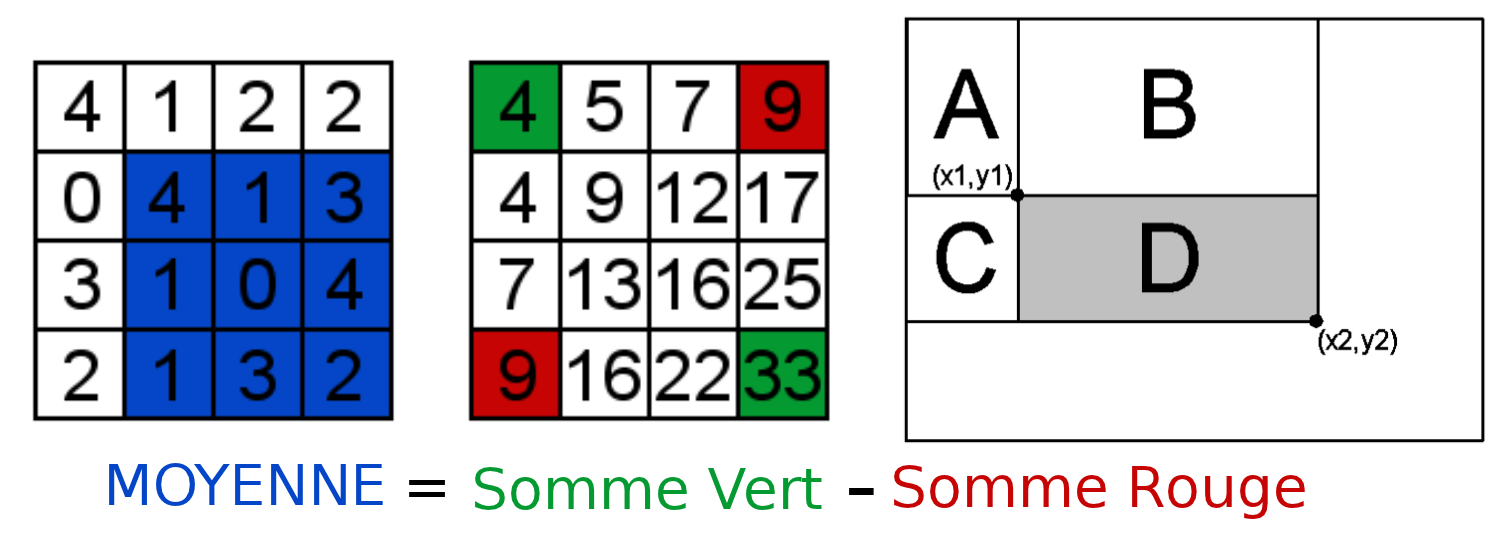
\includegraphics[width=\textwidth]{images/imageIntegrale.png}
\end{center}
%article de ...
%permet d'obtenir la moyenne en 2 additions et deux soustractions

\end{frame}

%% part 3 - Nicolas
\section[Détection de Pictogrammes]{Détection de Pictogrammes}
\begin{frame}{Objectif}
\vspace{5mm}
\begin{block}{}
\begin{itemize}
\item Développer un logiciel qui détecte des pictogrammes dans un flux vidéo.
\item Utilisation de templates représentant les pictogrammes.
\end{itemize}
\end{block}
\begin{center}
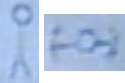
\includegraphics[scale=0.66]{images/templates.png}
\end{center}
\end{frame}

\begin{frame}{Méthode utilisée}
\vspace{5mm}
\begin{block}{}
Nous avons utilisé la méthode de Template Matching.
\end{block}
\begin{itemize}
\item Principe : 
\begin{center}
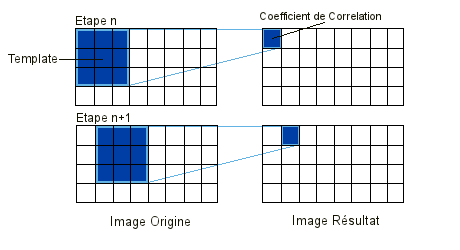
\includegraphics[scale=0.66]{images/templateMatching.png}
\end{center}
\end{itemize}
\end{frame}
			
\begin{frame}{Problème rencontré}
\vspace{5mm}
\begin{block}{}
Un problème rencontré est la présence de faux positifs.
\end{block}
\begin{itemize}
\item \texttt{cvMatchTemplate} -> Carte de corrélation
\item Récupération du meilleur résultat
\item Difficulté pour déterminer un seuil d'acceptation
\end{itemize}
\end{frame}	

\begin{frame}{Résultats obtenus}
\vspace{5mm}
\begin{center}
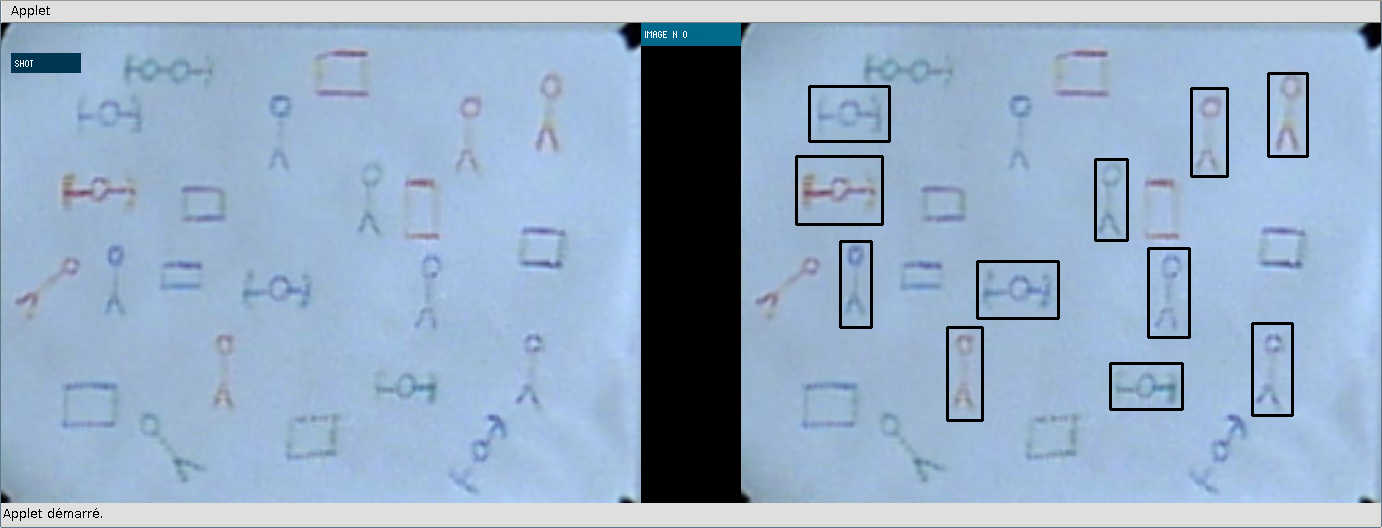
\includegraphics[width=\textwidth]{images/capture1.png}
\end{center}
\end{frame}

\begin{frame}{Résultats obtenus}
\vspace{5mm}
\begin{center}
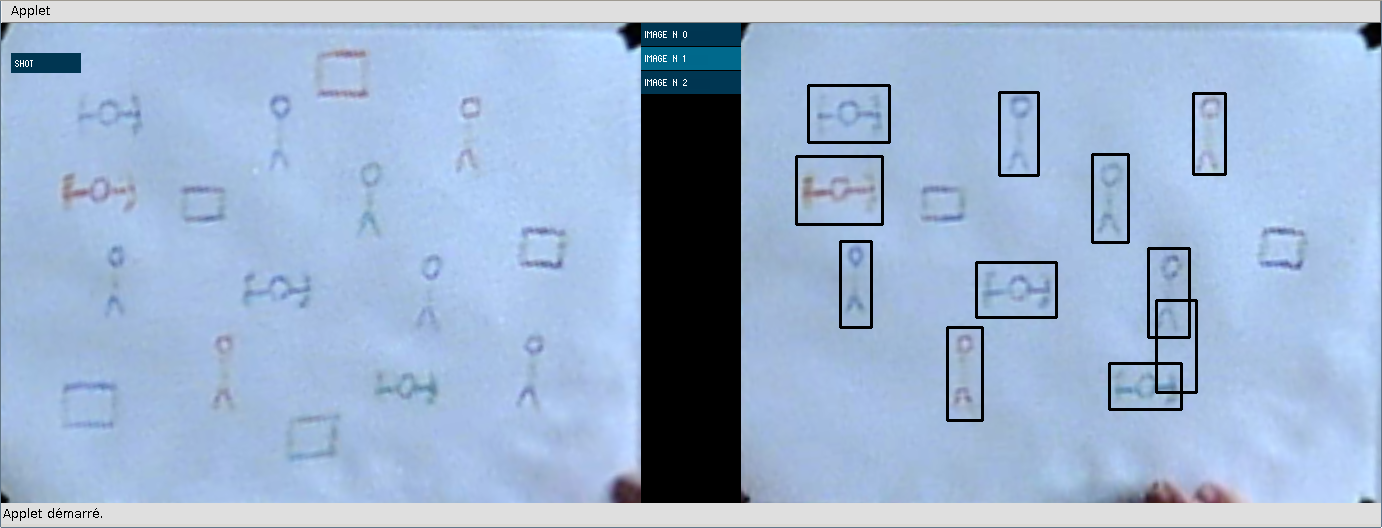
\includegraphics[width=\textwidth]{images/capture2.png}
\end{center}
\end{frame}

\begin{frame}{Méthode alternative}
\vspace{5mm}
\begin{block}{}
Nous avons également envisagé d'utiliser SURF.
\end{block}
\begin{itemize}
\item SURF : Speeded-Up Robust Features
\item Intérêt : Non affecté par rotation et mise à l'échelle 
\item Problème : Qualité vidéo trop basse -> Trop peu de marqueurs détectés
\end{itemize}
\end{frame}
	%% part 4 - Tomy
\section[Extraction de nouveautés]{Feature Extractor}
\begin{frame}{Objectif}
\vspace{5mm}
\begin{block}{}
\begin{itemize}
\item Développer un logiciel qui permet de voir l'évolution d'un dessin.
\end{itemize}
\end{block}
\begin{center}
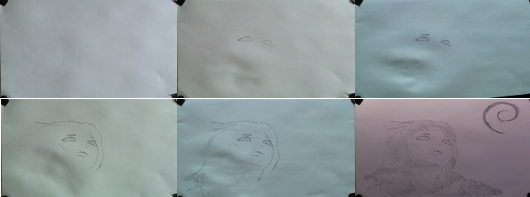
\includegraphics[width=\textwidth]{images/evo/evo.png}
\end{center}
\end{frame}

\begin{frame}{Tâtonnement}
\vspace{5mm}
\begin{block}{}
Dans un premier temps nous avons fait une simple différence d'images.
\end{block}
\begin{center}
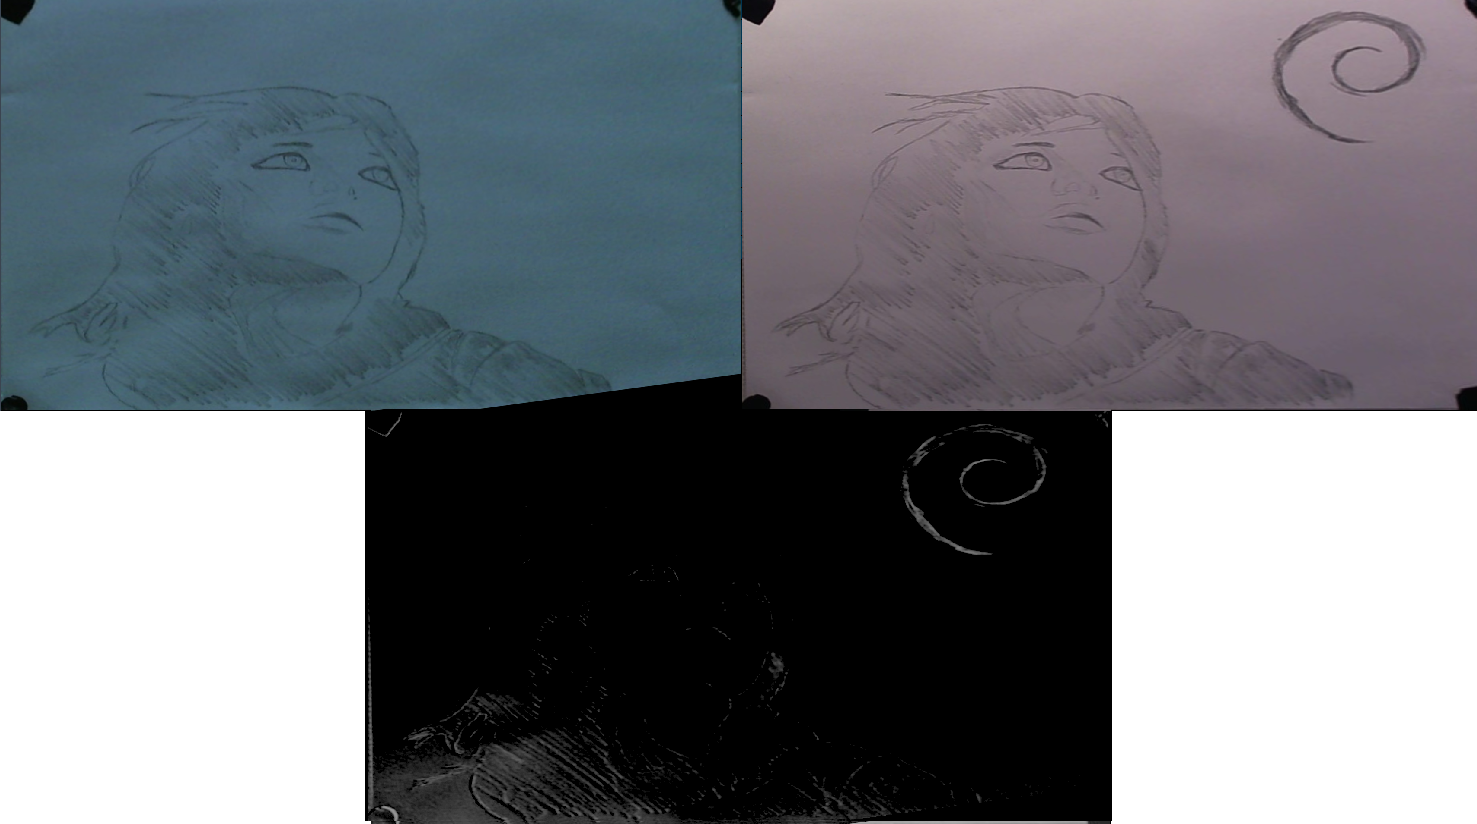
\includegraphics[width=\textwidth]{images/evo/diff.png}
\end{center} 
\end{frame}

\begin{frame}{Tâtonnement}
\vspace{5mm}
\begin{block}{}
Dans un premier temps nous avons fait une simple différence d'images.
\end{block}
\vspace{5mm}
\begin{itemize}
\item Problème : Impossible d'extraire les nouveautés
\item Solution : \'Etape de pré-traitement
\end{itemize}
\end{frame}

\begin{frame}{Caractéristiques des images}
\vspace{5mm}
\begin{block}{}
Les images que nous avons présentent des défauts.
\end{block}

\begin{itemize}
\item Coloration : 
	\begin{itemize}
	\item Le dessin est un processus long
	\item Rend l'analyse plus difficile
	\item Nécessité d'une balance des blancs
	\end{itemize}
\item Haute qualité :
	\begin{itemize}
	\item Rend l'analyse plus facile
	\item Augmente le temps d'analyse
	\item Algorithme efficace nécessaire
	\end{itemize}
\end{itemize}
\end{frame}

\begin{frame}{Méthode utilisée}
\vspace{5mm}
\begin{block}{}
\textbf{Idée :} extraction d'un masque de nouveautés
\end{block}
\begin{itemize}
\item Binarisation des images
\item Différence des images obtenues
\end{itemize}
\end{frame}

\begin{frame}{Résultats obtenus}
\vspace{5mm}
\begin{center}
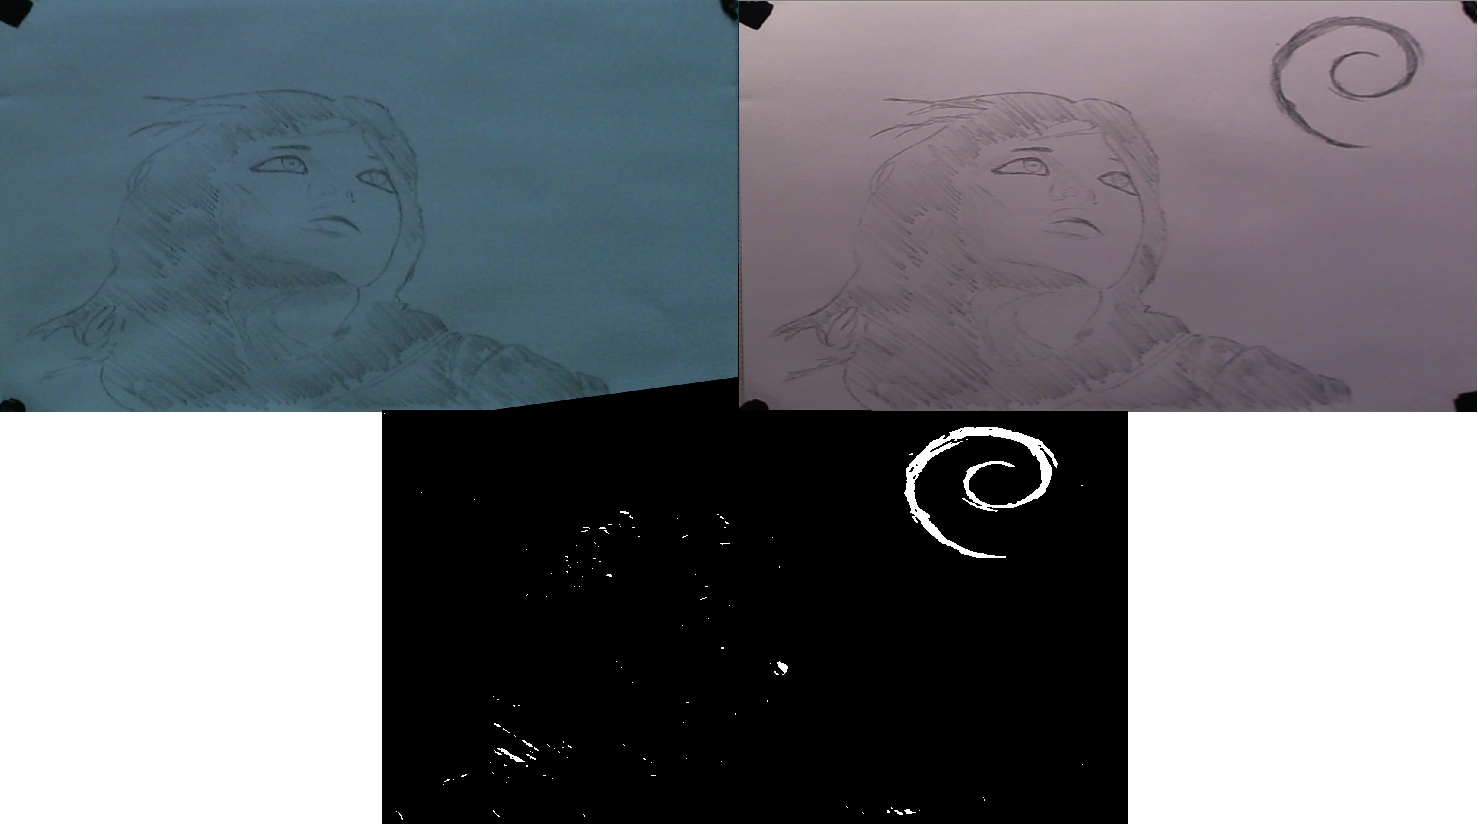
\includegraphics[width=\textwidth]{images/evo/masque.png}
\end{center}
\end{frame}


\begin{frame}{Résultats obtenus}
\vspace{5mm}
\begin{center}
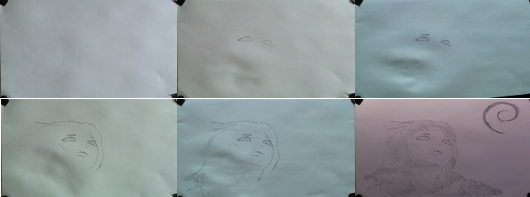
\includegraphics[width=\textwidth]{images/evo/evo.png}
\end{center}
\end{frame}
\begin{frame}{Résultats obtenus}
\vspace{5mm}
\begin{center}
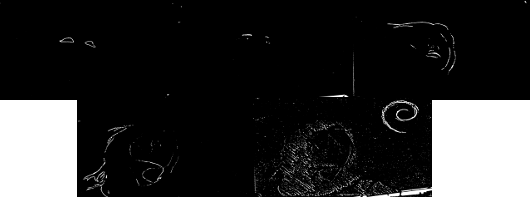
\includegraphics[width=\textwidth]{images/evo/evomasque.png}
\end{center}
\end{frame}
			
\begin{frame}{Problème rencontré}
\vspace{5mm}
\begin{block}{}
Il est difficile de supprimer totalement le bruit sur le masque
\end{block}
\begin{itemize}
\item Différence de recalage
\item Le dessinateur redessine par dessus
\end{itemize}
\end{frame}	


\section[Conclusion]{Conclusion}
	\begin{frame}{Conclusion}
		\vspace*{5mm}
		\begin{itemize}
		\item Objectifs partiellement atteints
		\begin{itemize}
		\item Filtrage par couleur
		\end{itemize}
		\item Résultats obtenus acceptables
		\item Piste d'évolution:
		\begin{itemize}
		\item Amélioration des détecteurs
		\item Vectorisation du dessin pour la détection de nouveautés
		\end{itemize}
		\end{itemize}
	\end{frame}

\end{document}
